% importa variabili globali
% definizione variabili globali
\def\GRUPPO {Stark Labs}

\def\PROGETTO {\textbf{SiVoDiM}}

\def\COMMITTENTE {Prof. Tullio Vardanega, \\ & Prof. Riccardo Cardin}

\def\PROPONENTE {Giulio Paci, MIVOQ s.r.l.}

\def\AZIENDA {MIVOQ s.r.l.}

\def\EMAIL {starklabs.swe@gmail.com}

\def\LOGO {../template/img/logo.png}

\def\INTESTAZIONE {../template/img/intestazione.png}
\def\PIEDIPAGINA {../template/img/piedipagina.png}

\def\G {{\small $_G$}}


% definizione variabili locali
\def\DOCUMENTO{Piano di Progetto}
\def\VERSIONE{1.0.0}

\def\DESCRIZIONE{<Info documento>}

\def\REDATTORE {Alberto Andriolo\\ & Francesco Bizzaro}
\def\VERIFICATORE {Riccardo Rizzo}
\def\RESPONSABILE {Enrico Chiara}

\def\USO {Esterno}

\def\DISTRIBUZIONE {\GRUPPO{}\\ & \COMMITTENTE{}\\}

\def\DESCRIZIONE {Documento riguardante la pianificazione del progetto \PROGETTO}


% abilita (true) / disabilita (false) indice, lista tabelle, lista figure
\def\INDICE	{true}
\def\TABELLE {true}
\def\FIGURE {true}


% importa struttura
\documentclass[a4paper]{article}

% ----- definizioni -----
\def\TITLE		{\mbox{\GRUPPO}}
\def\SUBTITLE	{\SIGLA, \PROGETTO}


% ----- nuovi comandi -----
% fornisce il caption per riferirsi ad una particolare sezione
\newcommand{\numref}[1]{\textsf{\textsl{``\nameref{#1}'' (\ref{#1})}}}


% ----- package -----
\usepackage[T1]{fontenc}   % codifica dei font in uscita

%prove_font
\usepackage[default]{gillius}
\renewcommand{\familydefault}{\sfdefault}
%\usepackage{times}
%\textsf{Arial}
%end_prove_font

\usepackage[utf8]{inputenc}   % lettere accentate da tastiera
\usepackage[italian]{babel}   % lingua principale del documento
\usepackage[a4paper, top= 3cm, bottom= 3cm, left= 3cm, right= 3cm, bindingoffset= 5mm]{geometry} % impostazione margini

\usepackage{amssymb} %

\usepackage{booktabs} % comandi aggiuntivi per le tabelle

\usepackage{calc} % espressioni aritmetiche
\usepackage{caption} % descrizione figure, ecc
\usepackage{chapterbib} % inclusione delle bibliografie

\usepackage{datatool} % manipolazione dati
\usepackage{dcolumn} % array in tabular

\usepackage{epstopdf} % conversione eps--> pdf
\usepackage{enumitem} % personalizzazione liste
\usepackage{eurosym} % simbolo euro

\usepackage{fancyhdr}   %personalizzazione dello stile
\usepackage{float} % definizione di oggetti floating (es. figure, tabelle)
\usepackage[bottom]{footmisc} % personalizzazione note

\usepackage[]{glossaries}	% glossario
\usepackage{graphicx, subfigure} % pacchetto grafica testo
\usepackage{grffile} % estende gestione filename graphic

\usepackage[colorlinks=true, urlcolor=blue, citecolor=black, linkcolor=black, hyperindex, breaklinks]{hyperref} % gestione dei link

\usepackage{ifthen}	% costrutto ifthenelse

% \usepackage{listings} % inserimento pezzi di codice
\usepackage{longtable} % tabelle su più pagine

\usepackage{pgf} % grafica postscript e PDF
\usepackage{pgfplots}	% composizione di grafici
\pgfplotsset{/pgf/number format/use comma, compat=newest}	% opzioni per i grafici

\usepackage{multirow} % span multiriga

\usepackage{tabularx, array} % crea paragrafi a colonne
\usepackage{titlesec} % personalizzazione titoli
\usepackage{tikz} % gestione delle formule
\usepackage{totpages} % conta numero pagine

\usepackage{soul} % gestione letterspacing
\usepackage{subfigure} % gestione delle sottofigure

\usepackage{verbatim} % inserimento testo verbatim, non interpretato

\usepackage{wallpaper} % gestione background

\usepackage{xspace} % spazi automatici per le macro


% ----- posizione etichette -----
\captionsetup{tableposition=top, figureposition=bottom, font=small}


% ----- glossario -----
%\loadglsentries{../../glossario/glossario.tex}
\renewcommand*{\glssymbolsgroupname}{Simboli}


% ----- stile pagina -----
\pagestyle{fancy}

	% header
	\fancypagestyle {firststyle} {	% definizione stile "firststyle"
		\fancyhf{}
	}

	% indentazione paragrafo
	%\setlength{\parindent} {0pt}
	\setlength{\headheight} {25pt}

	% intestazione
	\lhead{}
	\rhead{\nouppercase{\leftmark}}
	\renewcommand{\headrulewidth}{0pt}  % no linea sotto intestazione

	% piè di pagina
	\lfoot{\footnotesize{{\DOCUMENTO} \\ {\VERSIONE}}}
	\cfoot{}
	\rfoot{\thepage}
	\renewcommand{\footrulewidth}{0pt}   % no linea sopra piè di pagina


% ----- inizio documento -----

% ----- prima pagina -----
\begin{document}
\thispagestyle{firststyle}

\begin{center}

%   \vspace{7cm}
	\textbf{{\fontsize{40pt}{41pt}\selectfont \PROGETTO}} \\
	\rule{8cm}{3pt}
   
   \vspace{4cm}
   \includegraphics[height= 4cm] {\LOGO}
   
%	\vspace{1cm}
%   {\fontsize{30pt}{31pt}\selectfont \textbf{\GRUPPO}}
	
	\vspace{5cm}
	{\fontsize{18pt}{24pt}\selectfont \textbf{\DOCUMENTO}}
	
%	\vspace{1cm}
	\begin{center}
		\begin{tabular}{r|l}
				\textbf{Versione} & \VERSIONE \\
				\textbf{Redattori} & \REDATTORE \\
				\textbf{Verificatori} & \VERIFICATORE \\
				\textbf{Responsabili} & \RESPONSABILE \\
				\textbf{Uso} & \USO \\
				\textbf{Lista di distribuzione} & \DISTRIBUZIONE
		\end{tabular}
	\end{center}

	\vspace{1cm}
	\textbf{\DESCRIZIONE}

\end{center}


\newpage

% ----- pagine successive -----
\ULCornerWallPaper{1}{\INTESTAZIONE}
\LLCornerWallPaper{1}{\PIEDIPAGINA}

%\thispagestyle{empty}

\newpage

% diario delle modifiche


% numerazione pagine indici
\pagenumbering{Roman}


\vspace{1cm}
   {\fontsize{15pt}{16pt}\selectfont \textbf{Registro delle modifiche}}\\ \\

\bgroup
\def\arraystretch{1.6}
\begin{tabular}{| c | c | c | c |}
\hline
\textbf{Attività} & \textbf{Autori} & \textbf{Data} & \textbf{Versione}\\ \hline \hline

%  ATTIVITA` & AUTORI & DATA & VERSIONE \\ \hline

Accettazione & Enrico Chiara & 31/03/2016 & 1.0.0 \\ \hline 

Verifica & Riccardo Rizzo & 30/03/2016 & 0.2.0 \\ \hline

Correzione errori & Alberto Andriolo & 30/03/2016 & 0.1.1 \\ \hline

Verifica & Riccardo Rizzo & 30/03/2016 & 0.1.0 \\ \hline 

Stesura preventivo & Alberto Andriolo & 23/03/2016 & 0.0.5 \\ \hline 

Stesura pianificazione RP e RQ e RA & Francesco Bizzaro & 21/03/2016 & 0.0.4 
\\ \hline

Stesura pianificazione AR e AD & Albero Andriolo & 14/03/2016 & 0.0.3 \\ 
\hline 

Stesura rischi di progetto & Francesco Bizzaro & 11/03/2016 & 0.0.2 \\ \hline 

Creazione documento & Francesco Bizzaro & 11/03/2016 & 0.0.1 \\ \hline 

% fine contenuti tabella

\end{tabular}
\egroup
\newpage

% importa indici
% definizione indice
\ifthenelse{\equal{\INDICE}{true}}
	{\setcounter{secnumdepth}{5}
\setcounter{tocdepth}{5}
	\tableofcontents \newpage}{}

% definizione lista tabelle
\ifthenelse{\equal{\TABELLE}{true}} 
	{\listoftables \newpage}{}

% definizione lista figure
\ifthenelse{\equal{\FIGURE}{true}}
	{\listoffigures \newpage}{}


% numerazione pagine
\pagenumbering{arabic}

	% formato visualizzazione
	\rfoot{\thepage ~di~\pageref{TotPages}}


% separatore
\iffalse
	AOjvdYTJD7mcIIYItfsNiYPbmTTogRSP9hrrb2XPE1laMyQ9NHrPgTCTxnW0eV1YcM3Wqh7t5qThjczeXWq3O5FJ7BBQjoWZovC5
\fi

% importa parti documento

\section{Organigramma}

\subsection{Redazione}
\begin{table}[h]
\centering
\bgroup
\def\arraystretch{3}
\begin{tabular}{| c | c | p{5cm} |}
\hline
\textbf{Nominativo} & \textbf{Data di Redazione} & \textbf{Firma}\\ \hline 
\hline
Responsabile & 01/04/2016 & 
%\includegraphics[width=4cm]%{immagini/firma_alberto.png}
\\ \hline  
\end{tabular}
\egroup
\caption{Redazione}
\end{table}

\subsection{Approvazione}
\begin{table}[h]
\centering
\bgroup
\def\arraystretch{3}
\begin{tabular}{| c | c | p{5cm} |}
\hline
\textbf{Nominativo} & \textbf{Data di Approvazione} & \textbf{Firma}\\ \hline \hline
Responsabile & 01/04/2016 & 
%\includegraphics[width=4cm]{immagini/firma_alberto.png}
\\ \hline  
Docente &  & \\ \hline
\end{tabular}
\egroup
\caption{Approvazione}
\end{table}

\newpage

\subsection{Accettazione dei componenti}
\begin{table}[h]
\centering
\bgroup
\def\arraystretch{3}
\begin{tabular}{| c | c | p{5cm} |}
\hline
\textbf{Nominativo} & \textbf{Data di Approvazione} & \textbf{Firma}\\ \hline \hline
Alberto Andriolo & 03/03/2016 & 
%\includegraphics[width= 4cm]{png/firma_alberto.png}
\\ \hline  
Enrico Chiara & 03/03/2016 & 
%\includegraphics[width=4cm]{png/firma_enrico.png}
\\ \hline
Federico Rossetto & 03/03/2016 & 
%\includegraphics[width=4cm]{png/firma_federico.png}
\\ \hline
Francesco Bizzaro & 03/03/2016 & 
%\includegraphics[width=4cm]{png/firma_francesco.png}
\\ \hline
Gino Zaidan & 03/03/2016 & 
%\includegraphics[width= 4cm]{png/firma_gino.png}
\\ \hline
Riccardo Rizzo & 03/03/2016 & 
%\includegraphics[width=4cm]{png/firma_riccardo.png}
\\ \hline
\end{tabular}
\egroup
\caption{Accettazione}
\end{table}

\newpage

\subsection{Componenti del gruppo}
Il \textit{team} \GRUPPO\ è composto dei seguenti membri:
\begin{table}[h]
\centering
\bgroup
\def\arraystretch{1.6}
	\begin{tabular}{| c | c | c |}
		\hline
		\textbf{Nominativo} & \textbf{Matricola} & \textbf{Indirizzo di posta 
		elettronica} \\ \hline \hline 
		Alberto Andriolo & 1074665 & alberto.andriolo.1@studenti.unipd.it 
		\\ \hline
		Enrico Chiara & 1005608 & enricochiara@icloud.com \\ \hline
		Federico Rossetto & 1031919 & federico.rossetto@studenti.unipd.it \\ 
		\hline
		Francesco Bizzaro & 1069586 & francescob994@gmail.com  \\ \hline  
		Gino Zaidan & 1008249 & zaidan90@hotmail.it  \\ \hline 
		Riccardo Rizzo & 1054776 & rizzoricky@gmail.com  \\ \hline
	\end{tabular}
\egroup
\caption{Componenti}
\end{table}

\subsection{Ruoli}
Ogni componente del gruppo deve poter sperimentare tutte le categorie di attività previste in ambito progettuale. Pertanto devono essere scambiati a rotazione fra i membri del \textit{team} i seguenti ruoli:
\begin{table}[h]
\centering
\bgroup
\def\arraystretch{1.6}
\begin{tabular}{| c | c |}
\hline
\textbf{Ruolo} & \textbf{Costo (euro/ora)}\\ \hline \hline
Responsabile & 30  \\ \hline 
Amministratore & 20  \\ \hline 
Analista & 25  \\ \hline 
Progettista & 22  \\ \hline 
Programmatore & 15  \\ \hline
Verificatore & 15  \\ \hline  
\end{tabular}
\egroup
\caption{Ruoli e costi}
\end{table}

\newpage
\section{Introduzione}

\subsection{Scopo del documento}
Questo documento ha lo scopo di descrivere l'organizzazione che il gruppo \GRUPPO\ si impegna ad attuare per portare a termine il progetto \PROGETTO. Viene pianificata, sulla base delle scadenze e delle risorse disponibili, la dislocazione temporale con cui suddividere in modo proficuo le attività da svolgere. Più precisamente, viene indicato:
\begin{itemize}
\item Un insieme di fattori di rischio che sono stati identificati per poter essere arginati;
\item Il tempo previsto per ogni attività;
\item Una stima del costo in termini di risorse;
\item Un bilancio sull'utilizzo totale delle risorse.
\end{itemize}  

\subsection{Scopo del progetto}
Lo scopo del progetto risiede nello sviluppo di un'applicazione utile a dimostrare efficacemente
le potenzialità del motore di sintesi vocale FA-TTS\G, realizzato dall'azienda \AZIENDA\ e messo a disposizione del gruppo di lavoro. Si devono realizzare due applicazioni per sistemi Android\G:
\begin{itemize}
	\item \textbf{Applicazione di configurazione}: deve permettere all'utente di interfacciarsi direttamente con il sistema operativo per configurare, salvare e modificare le voci ereditate dal motore di sintesi FA-TTS di MIVOQ;
	\item \textbf{Applicazione per la creazione di sceneggiati}: permette la creazione e il salvataggio di racconti e sceneggiati, che possono essere esportati in formato audio attraverso l'utilizzo del motore FA-TTS.
\end{itemize}
Entrambe le applicazioni devono interfacciarsi con due moduli di basso livello:
\begin{itemize}
	\item \textbf{Modulo di sistema}: permette di interfacciarsi tramite connessione di rete al motore FA-TTS;
	\item \textbf{Libreria}: una libreria contenente tutte le funzionalità offerte dal motore FA-TTS, utile nell'ottica di un riuso futuro del \textit{software}.
\end{itemize} 
Lo sviluppo di tutte e quattro le suddette componenti è a carico del gruppo Stark Labs.

\subsection{Glossario}
Al fine di aumentare la comprensione del testo ed evitare eventuali ambiguità, 
viene fornito un glossario (\textit{Glossario v1.0.0}) contenente le 
definizioni degli acronimi e dei termini tecnici utilizzati nel documento. Ogni 
vocabolo contenuto nel glossario è contrassegnato dal pedice "\G ".

\subsection{Riferimenti}

\subsubsection{Normativi}
\begin{itemize}
\item \textit{Norme di Progetto v1.0.0};
\item \textbf{Regole del progetto didattico}: \url{http://www.math.unipd.it/~tullio/IS-1/2015/Dispense/PD01.pdf};
\item \textbf{Regolamento Organigramma}: \url{http://www.math.unipd.it/~tullio/IS-1/2015/Progetto/PD01b.html}.
\end{itemize}

\subsubsection{Informativi}
\begin{itemize}
\item \textit{Glossario v1.0.0};
\item \textit{Studio di Fattibilità v1.0.0}.
\item \textbf{SWEBOK Guide\G}: The Guide to the Software Engineering Body of Knowledge V3 \\ \url{https://www.computer.org/web/swebok/}
\end{itemize}
 

\subsection{Scadenze}
Di seguito sono riportate le scadenze che il gruppo \GRUPPO\ si impegna a rispettare. La fase di pianificazione delle attività si basa su tali date:
\begin{itemize}
\item \textbf{Revisione dei Requisiti (RR)}: 18/04/2016;
\item \textbf{Revisione dei Progettazione (RP)}: 23/05/2016;
\item \textbf{Revisione di Qualifica (RQ)}: 17/06/2016;
\item \textbf{Revisione di Accettazione (RA)}:  11/07/2016.
\end{itemize}

\subsection{Ciclo di vita}
Per lo sviluppo del prodotto è stato scelto di seguire il \textbf{modello di ciclo di vita incrementale}. Questo consente di spezzare la realizzazione delle componenti richieste in periodi temporali distinti, alla cui fine è prevista una specifica fase di verifica. In questo modo si garantisce un controllo attento e dettagliato per ogni fase. Una forte suddivisione infatti consente di applicare più facilmente il ciclo di Deming\G, garantendo un forte controllo sull'andamento del progetto. Inoltre questo modello consente di focalizzarsi inizialmente sui requisiti principali, lasciando l'implementazione di tutti gli altri requisiti (secondari) a un secondo momento. I motivi principali per cui è stato scelto questo modello sono:
\begin{itemize}
\item La struttura del prodotto richiesto, composto di componenti distinte con un diverso grado di importanza per il Proponente;
\item La grande disponibilità del Proponente a discutere con il \textit{team}, anche durante lo sviluppo (mediante incontri o conferenze audio);
\item La possibilità di spezzare il lavoro in più fasi, in cui dedicarsi alla risoluzione di specifici requisiti per incrementi successivi;
\item Maggiore controllo sull'avanzamento del progetto dato dalla facilità di applicare il ciclo di Deming\G\ su fasi di breve durata;
\item La possibilità di fare prototipi, o usare una versione precedente del prodotto, per chiedere al Proponente delucidazioni riguardo il soddisfacimento di requisiti;
\item La possibilità di eseguire test di maggiore dettaglio, dedicati al prodotto di ciascuna fase;
\item Il vantaggio di procedere nel lavoro concentrandosi da subito sugli obiettivi strategici obbligatori e solo in un secondo momento su quelli opzionali, riducendo il rischio di un fallimento completo del progetto.
\end{itemize}

\newpage
\section{Analisi dei rischi}
Per tutta la durata dello sviluppo del progetto, è sempre possibile il verificarsi di eventi che possono rallentare o far deviare l'andamento delle fasi di lavoro pianificate. Per evitare di incorrere in queste problematiche viene eseguita un'analisi dei rischi, che prevede i seguenti punti:
\begin{itemize}
\item Identificazione del rischio;
\item Calcolo della probabilità che si verifichi;
\item Stima della gravità in caso di occorrenza;
\item Identificazione di un metodo di controllo che possa informare per tempo i componenti del gruppo sul verificarsi del rischio calcolato;
\item Pianificazione di contromisure che possano gestire o prevenire l'avverarsi del problema.
\end{itemize}
Di seguito sono descritti i rischi identificati, raggruppati per ambito in sotto-sezioni distinte.

%---------------------------------------------------------------------------------
\subsection{Rischi relativi ai requisiti}

\subsubsection{Requisito non rilevato}
\label{sec:ReqNonRil}
L'analisi dei requisiti potrebbe non essere completa e tralasciare alcuni requisiti ritenuti importanti dal proponente\G. Dato che il capitolato lascia parecchia libertà al \textit{team}, non specificando quale dovrà essere l'applicazione \textit{mobile} da sviluppare (si veda lo Studio di Fattibilità v1.0.0), sarà molto probabile incorrere in questa problematica. 
\begin{itemize}
\item \textbf{Probabilità}: Alta;
\item \textbf{Grado di pericolosità} Alto;
\item \textbf{Controllo}: Per verificare che i requisiti rilevati soddisfino il proponente\G, durante la fase di analisi vengono fatti degli incontri - se possibile - o in alternativa lo si contatta attraverso la mail ufficiale, chiedendo conferma di quanto ricavato;
\item \textbf{Contromisure}: Non vi è modo di eliminare del tutto questo rischio, ma il colloquio con il proponente\G\ lo abbassa significativamente. Per minimizzarlo si farà particolare attenzione nella fase di verifica del documento dell'Analisi dei Requisiti.
\end{itemize}

%---------------------------------------------------------------------------------
\subsection{Rischi tecnologici}

\subsubsection{Scarsa conoscenza delle tecnologie scelte}
\label{sec:ScarsTec}
I membri del \textit{team} non hanno esperienze sulla tecnologia TTS\G\ né sullo sviluppo in ambiente \textit{mobile}. Questo ritarderà la fase iniziale in cui è necessario inserire una fase di apprendimento.
\begin{itemize}
\item \textbf{Probabilità}: Alta;
\item \textbf{Grado di pericolosità}: Medio;
\item \textbf{Controllo}: il Responsabile di Progetto ha il compito di verificare il grado di conoscenza di ciascun membro del \textit{team} sulle tecnologie necessarie al completamento del suo ruolo;
\item \textbf{Contromisure}: L'unico modo di procedere è reperire informazioni sugli argomenti in questione e provvedere affinché ciascun componente del \textit{team} possa acquisire sufficienti informazioni. Non vi è modo di non spendere del tempo per questa fase.
\end{itemize}

\subsubsection{Malfunzionamento del servizio di personalizzazione della voce}
\label{sec:PMalf}
Mivoq srl mette a disposizione un servizio di personalizzazione della voce, che permette all'utente di creare la propria voce digitale, utilizzabile in seguito dal motore di sintesi. Questo servizio è offerto attraverso una piattaforma web, e al momento è in fase di \textit{beta testing}\G. L'utilizzo di un servizio sperimentale e non ancora testato può costituire un rischio per il progetto.
\begin{itemize}
\item \textbf{Probabilità}: Bassa;
\item \textbf{Grado di pericolosità}: Bassa;
\item \textbf{Controllo}: Se questo servizio verrà utilizzato dall'applicazione che deve essere sviluppata, saranno effettuati dei test mirati a verificare il corretto funzionamento del servizio;
\item \textbf{Contromisure}: In caso di problemi di qualsiasi genere, riguardanti questo servizio, Mivoq srl si impegna a fornire assistenza al \textit{team}. 
\end{itemize} 

\subsubsection{Problemi Software}
\label{sec:PSW}
Per migliorare la produttività si fa uso di \textit{software}\G\ esterno di vario genere, che potrebbe corrompersi, risultare insicuro o rivelarsi inaffidabile.
\begin{itemize}
\item \textbf{Probabilità}: Bassa;
\item \textbf{Grado di pericolosità}: Medio;
\item \textbf{Controllo}: Giornalmente l'Amministratore del gruppo deve controllare il corretto funzionamento degli applicativi web utilizzati. In aggiunta ogni membro del \textit{team} è tenuto a segnalare immediatamente eventuali malfunzionamenti, nel caso si verificassero;
\item \textbf{Contromisure}: In caso un membro del gruppo riscontrasse problemi di funzionamento negli applicativi utilizzati in locale, è tenuto all'aggiornamento o reinstallazione degli stessi. \\ 
Per minimizzare i problemi legati al rischio che venissero meno i servizi web utilizzati, invece, vengono eseguite periodicamente delle copie di backup dei dati remoti.
\end{itemize}

\subsubsection{Problemi Hardware}
\label{sec:PHW}
Il progetto è sviluppato su macchine che i membri del \textit{team} utilizza anche per scopi personali. Sono possibili guasti e danneggiamenti, che possono portare alla perdita di dati.
\begin{itemize}
\item \textbf{Probabilità}: Bassa;
\item \textbf{Grado di pericolosità}: Medio;
\item \textbf{Controllo}: Ciascun componente del \textit{team} ha cura della propria attrezzatura di lavoro, e la controlla periodicamente;
\item \textbf{Contromisure}: Per minimizzare la possibilità di perdere dati, ogni membro del gruppo deve eseguire il \textit{push} sul \textit{repository\G} al termine di ogni sessione lavorativa. \\
In caso un componente del \textit{team} fosse impossibilitato a lavorare con la propria macchina a seguito di un guasto, egli potrà utilizzare il proprio \textit{account} di laboratorio nella sede universitaria, per il tempo necessario alla riparazione della stessa.
\end{itemize}

%---------------------------------------------------------------------------------
\subsection{Rischi riguardanti il gruppo}

\subsubsection{Assenze per problemi personali o di salute}
\label{sec:Assenze}
Ogni componente del gruppo potrebbe ammalarsi o doversi assentare per impegni personali, dedicando meno tempo al progetto di quanto previsto, in certe occasioni. Ci sono anche studenti pendolari che potrebbero avere problemi di trasporto.
\begin{itemize}
\item \textbf{Probabilità}: Media;
\item \textbf{Grado di pericolosità}: Medio;
\item \textbf{Controllo}: Ogni impegno personale deve essere comunicato prontamente al Responsabile di Progetto, con quanto più preavviso possibile. Lo stesso vale in caso di imprevisti;
\item \textbf{Contromisure}: Non è possibile eliminare il rischio di imprevisti e malattia, ma è possibile minimizzarlo con opportune precauzioni da parte dei componenti del \textit{team}. \\
Il Responsabile di progetto a fronte di una comunicazione di impegni vari o problematiche, deve al più presto stilare un novo piano per sopperire alla mancanza della persona.
\end{itemize}

\subsubsection{Incomprensioni fra componenti}
\label{sec:Incomp}
Il \textit{team} è formato da sei persone con esperienze diverse ed eterogenee, che sono alla prima esperienza di lavoro collaborativo così numeroso. Ne consegue il rischio di incomprensioni o dissidi che potrebbero venire a formarsi, e andrebbero a incidere sia sull'efficienza che sulla qualità lavorativa.
\begin{itemize}
\item \textbf{Probabilità}: Bassa;
\item \textbf{Grado di pericolosità}: Alto;
\item \textbf{Controllo}: Il Responsabile di progetto ha il dovere di monitorare il clima lavorativo e il grado di cooperazione fra i membri del gruppo. Inoltre ciascuno è tenuto a fargli rapporto, in caso si verificassero conflitti di ogni sorta;
\item \textbf{Contromisire}: Ogni componente del \textit{team} è tenuto a collaborare con gli altri. Nel caso questo risultasse impossibile il Responsabile di Progetto deve mediare fra le parti per ridurre i contrasti.
\end{itemize}


%---------------------------------------------------------------------------------
\subsection{Rischi a livello organizzativo}

\subsubsection{Inesperienza lavorativa}
\label{sec:IneLav}
Essendo il primo lavoro cooperativo che i componenti del \textit{team} affrontano, possono sorgere problemi organizzativi, come difficoltà nella pianificazione e nella distribuzione di ruoli e \textit{task}. 
\begin{itemize}
\item \textbf{Probabilità}: Alta;
\item \textbf{Grado di pericolosità}: Medio;
\item \textbf{Controllo}: Il responsabile di progetto deve accertarsi che ogni componente del gruppo possa apprendere le conoscenze necessarie a svolgere il proprio ruolo, e che il carico di lavoro assegnato sia sostenibile ed equo fra le parti.
\item \textbf{Contromisure}: Ogni componente del gruppo è tenuto a documentarsi ed essere in grado di utilizzare tutta la strumentazione utile all'esercizio del proprio ruolo. Lo studio deve essere fatto ottimizzando i tempi di lavoro.
\end{itemize} 

\subsubsection{Errori nella stima delle tempistiche}
\label{sec:ErrTemp}
Il tempo assegnato per ogni attività potrebbe essere stimato in eccesso o in difetto. Data la generale inesperienza dei membri del \textit{team}, al primo lavoro collaborativo, potrebbe facilmente essere commesso un errore di pianificazione di questo tipo. Una sovrastima porta a tempi morti fra due attività, con conseguente spreco di risorse e denaro. Al contrario sottostimare porta facilmente a ritardi e slittamenti delle fasi previste.
\begin{itemize}
\item \textbf{Probabilità}: Alta;
\item \textbf{Grado di pericolosità}: Alto;
\item \textbf{Controllo}: Si deve controllare spesso il grado di avanzamento di ogni attività per accertarsi sia conforme ai tempi preventivati. Per fare ciò ci si avvale a strumenti di \textit{ticketing}\G.
\item \textbf{Contromisure}: Per evitare l'accumulo di ritardi a cascata e conseguenti slittamenti, devono essere previsti, in fase di pianificazione, dei margini di tempo fra le attività, in modo da recuperare il ritardo e riuscire ugualmente a raggiungere le \textit{milestone}\G\ nel momento previsto. 
\end{itemize}

%---------------------------------------------------------------------------------
% se la tabella non sta nella pagina!
%\newpage 

\subsection{Riepilogo}
\begin{table}[h]
\centering
\bgroup
\def\arraystretch{1.6}
\begin{tabular}{| c | c | c |}
\hline
\textbf{Rischio} & \textbf{Probabilità} & \textbf{Pericolosità}\\ \hline \hline 
\hyperref[sec:ReqNonRil]{Requisito non rilevato} & Alta & Alta \\ \hline
\hyperref[sec:ErrTemp]{Errori nella stima delle tempistiche} & Alta & Alta \\ \hline
\hyperref[sec:Incomp]{Incomprensioni fra componenti} & Bassa & Alta \\ \hline
\hyperref[sec:ScarsTec]{Scarsa conoscenza delle tecnologie scelte} & Alta & Media \\ \hline
\hyperref[sec:IneLav]{Inesperienza lavorativa} & Alta & Media \\ \hline
\hyperref[sec:Assenze]{Assenze per problemi personali o di salute} & Media & Media \\ \hline
\hyperref[sec:PSW]{Problemi \textit{software}} & Bassa & Media \\ \hline
\hyperref[sec:PHW]{Problemi \textit{hardware}} & Bassa & Media \\ \hline
\hyperref[sec:PMalf]{Malfunzionamento del servizio di personalizzazione della voce} & Bassa & Bassa \\ \hline
\end{tabular}
\egroup
\caption{Rischi rilevati, ordinati per grado di pericolosità e probabilità di verificarsi}
\end{table}



\section{Pianificazione}
I diagrammi delle attività presenti in questa sezione sono stati rappresentati 
tramite l'uso di diagrammi di Gantt.

\subsection{Analisi dei Requisiti}
\textbf{Periodo:} 04/03/2016 - 31/03/2016\\
Questa fase prevedere la scelta e l'implementazione degli strumenti necessari 
per definire il \textit{repository}\G\ utilizzato dal \textit{team}\G, le 
norme di base per sviluppare una documentazione quanto più possibile omogenea e 
coerente, una pianificazione che guida lo sviluppo del progetto. Termina con 
la scadenza di consegna dell'offerta, cioè con la consegna della 
\textit{Revisione dei Requisiti}.\\\\
I ruoli attivi in questa fase sono:

\begin{itemize}
	\item Responsabile;
	\item Amministratore;
	\item Analista;
	\item Progettista;
	\item Verificatore.
\end{itemize}
Le attività da svolgersi in questa fase sono:
\begin{itemize}
	\item \textbf{Ricerca ed implementazione degli strumenti}: 
	l'\textit{Amministratore di Progetto} ha il compito di scegliere, 
	implementare e configurare gli strumenti necessari al lavoro del team. Deve 
	apprendere il funzionamento e fare formazione ai rimanenti membri del 
	\textit{team\G} di sviluppo;
	\item \textbf{Norme di Progetto}: attività svolta 
	dall'\textit{Amministratore di 
	Progetto}. Concordati con il \textit{team}\G\ gli strumenti da utilizzare, 
	si procede 	alla stesura di un serie di norme, che dovranno essere 
	rispettate dai membri del team per tutta la durata del progetto. Le norme 
	sono interne al \textit{team}\G\ e non legate al capitolato SiVoDiM;
	\item \textbf{Studio di fattibilità}: è compito degli \textit{Analisti} 
	valutare ogni capitolato e redarre uno Studio di fattibilità, dal quale si 
	delinea chiaramente quale capitolato è stato scelto e la motivazione che ha 
	guidato a tale scelta.
	\item \textbf{Piano di Progetto}: qui vengono pianificate le attività, 
	risorse e costi della gestione del \textit{team}\G. Poi riportate in modo 
	strutturato nel \textit{Piano di Progetto v1.0.0};
	\item \textbf{Analisi dei Requisiti}: gli \textit{Analisti} hanno 
	l'incarico di ricercare i requisiti e di redigere il documento 
	\textit{Analisi dei Requisiti v1.0.0}, con Diagrammi dei Casi D'Uso (UC\G). 
	Questa attività è poco legata	al proponente\G, data la natura vaga del 
	Capitolato\G\ fornito dall'azienda MIVOQ s.r.l.;
	\item \textbf{Piano di Qualifica}: descrizione su strategie di verifica e 
	validazione adottate. Documentate poi nel \textit{Piano di Progetto v1.0.0};
	\item \textbf{Glossario}: attività parallela alla stesura di tutti i 
	documenti sopracitati. Il \textit{Glossario v1.0.0} verrà aggiornato in 
	modo incrementale fino al completamento della documentazione;
	\item \textbf{Verbale incontri}: per analizzare i requisiti presentati nel 
	Capitolato \G\ vengono organizzati incontri, in seguito documentati con 
	verbali formali.
\end{itemize}

\newpage
\begin{figure}
	\centering
	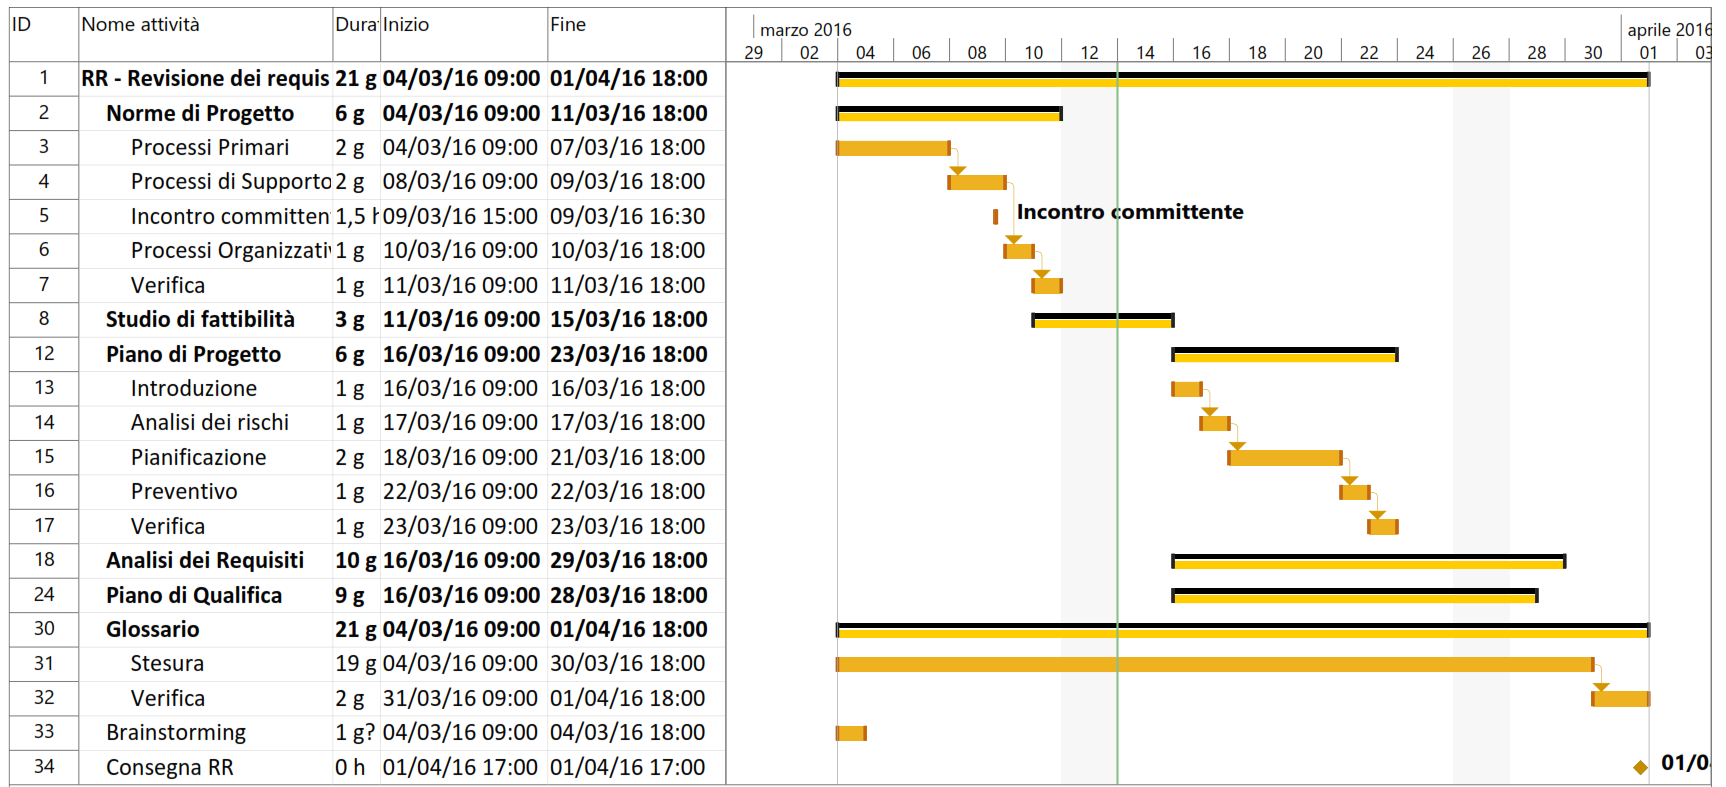
\includegraphics[width= 16cm]{AR.png}
	\caption{Analisi dei Requisiti}
\end{figure}


\subsection{Analisi di Dettaglio}
\textbf{Periodo:} 01/04/2016 - 18/04/2016\\
Questa attività ha termine con la presentazione in data 18/04/2016 dell'Analisi 
dei Requisiti\\\\
I ruoli attivi in questa fase sono:

\begin{itemize}
	\item Responsabile;
	\item Amministratore;
	\item Analista;
	\item Progettista;
	\item Verificatore.
\end{itemize}
Questa fase ha lo scopo di integrare e consolidare i requisiti ottenuti 
precedentemente.

\newpage
\begin{figure}
	\centering
	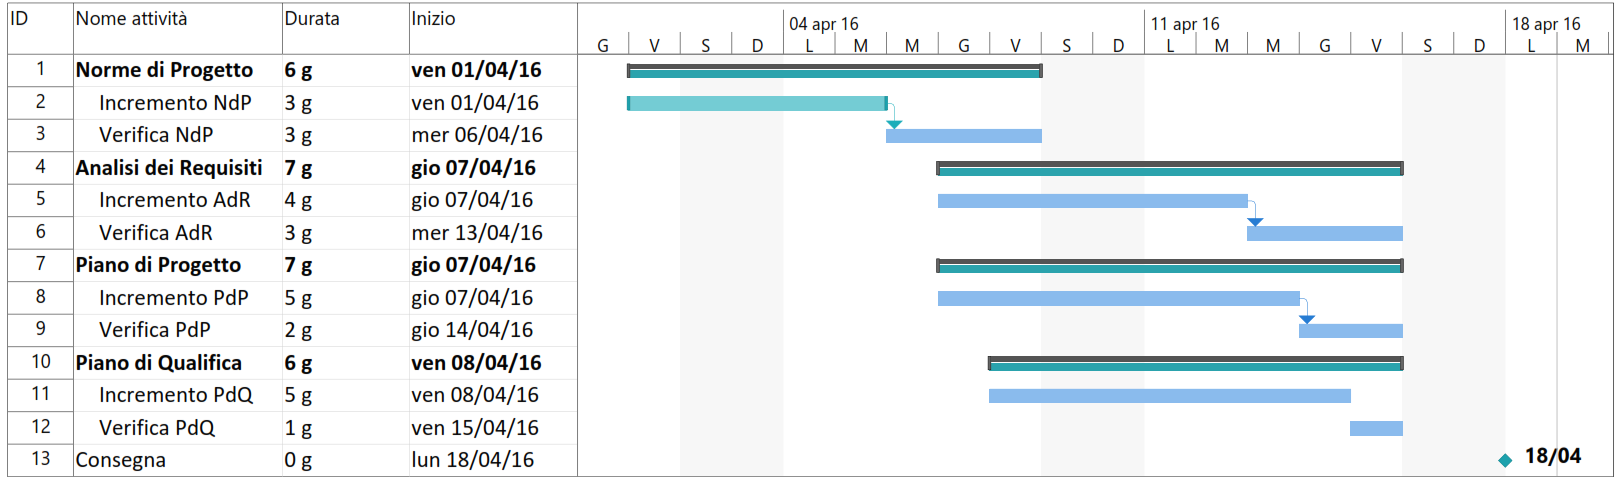
\includegraphics[width= 16cm]{AD.png}
	\caption{Analisi di Dettaglio}
\end{figure}

\subsection{Progettazione Architetturale}
\textbf{Periodo:} 19/04/2016 - 23/05/2016\\

\subsection{Progettazione di Dettaglio e Codifica}
\textbf{Periodo:} 24/05/2016 - 17/06/2016\\

\subsection{Validazione}
\textbf{Periodo:} 18/06/2016 - 11/07/2016\\
\input {sezioni/5_PdP.tex}
\input {sezioni/6_PdP.tex}

%\input {sections/nomesezione}
%\newpage

% ...

%\printglossaries

\end{document}
